% Arquivo principal: compilar main.tex com pdfLaTeX no Overleaf.
\documentclass[9pt,a4paper]{extarticle}
\usepackage[T1]{fontenc}
\usepackage[utf8]{inputenc}
\usepackage[brazil]{babel}
\usepackage{lmodern}
\usepackage[left=38pt,right=38pt,top=40pt,bottom=37pt,footskip=20pt]{geometry}
\usepackage{graphicx}
\usepackage[table]{xcolor}
\usepackage{array,tabularx,booktabs}
\usepackage{amsmath,amssymb}
\usepackage{titlesec}
\usepackage{fancyhdr}
\usepackage{microtype}
\usepackage{xurl}
\usepackage[unicode,hidelinks]{hyperref}

\definecolor{titulo}{HTML}{153D52}
\definecolor{cabecalho}{HTML}{E4EDF2}
\newcolumntype{Y}{>{\raggedright\arraybackslash}X}
\setlength{\parindent}{0pt}
\setlength{\parskip}{5pt}
\setlength{\emergencystretch}{2em}
\titleformat{\section}{\sffamily\bfseries\color{titulo}\fontsize{11.5}{15}\selectfont}{}{0pt}{}
\titleformat{\subsection}{\sffamily\bfseries\fontsize{9.8}{13}\selectfont}{}{0pt}{}
\titlespacing*{\section}{0pt}{6pt}{8pt}
\titlespacing*{\subsection}{0pt}{4pt}{5pt}
\pagestyle{fancy}
\fancyhf{}
\renewcommand{\headrulewidth}{0pt}
\fancyfoot[L]{\sffamily\fontsize{7}{9}\selectfont UNIVALI \textperiodcentered{} Sistemas em Tempo Real \textperiodcentered{} Atividade complementar M3}
\fancyfoot[R]{\sffamily\fontsize{7}{9}\selectfont\thepage}
\hypersetup{pdftitle={Quanto o teste enxerga do pior caso? -- Huffman na ESP32},pdfauthor={Miguel Bertonzin}}

\begin{document}
\fontsize{9}{12}\selectfont
% Conteúdo do relatório. Preencher o RA na identificação abaixo.

{\sffamily\bfseries\color{titulo}\fontsize{17}{21}\selectfont Quanto o teste enxerga do pior caso?\par}\vspace{9pt}

\section*{Codificação de Huffman na ESP32: quatro escopos de medição}

\textbf{Universidade do Vale do Itajaí --- UNIVALI | Escola Politécnica}
\par

Engenharia de Computação \textperiodcentered{} Sistemas em Tempo Real \textperiodcentered{} Atividade complementar M3 \textperiodcentered{} 2026
\par

\textbf{Acadêmico:} Miguel Bertonzin --- RA: [PREENCHER].
\par

\textbf{Professores:} Michael Douglas Cabral Alves e Felipe Viel.
\par

\textbf{Repositório:} \url{https://github.com/MiguelBertonzin/measurements-in-real-time-systems}
\par

\textbf{Campanha individual:} 13.000 ativações medidas na ESP32 de Miguel Bertonzin.
\par

\section*{1. Objetivo e delimitação}

Este trabalho investiga quanto o escopo de um teste altera o maior tempo de resposta observado de uma mesma tarefa. Foram realizadas quatro coletas de codificação de Huffman: tarefa isolada, atendimento de evento, concorrência entre tarefas e sistema com tráfego externo. A campanha reúne 13.000 ativações reais: 1.000 em cada uma das três primeiras etapas e 10.000 na quarta. As análises seguem as seções 3--9 do enunciado [1].
\par

O HWM (High Water Mark) é o máximo da amostra. Ele fornece uma aproximação potencialmente otimista do pior tempo de resposta, WCRT: observar um máximo não demonstra que nenhum estado futuro produzirá tempo maior. A questão central é separar cobertura da lógica, interferência temporal e tolerância a perdas. Para esta última, examinamos percentual no prazo, distâncias entre perdas, rajadas e o modelo (m,k)-firme.
\par

\section*{2. Plataforma, entrada e instrumentação}

\textbf{Plataforma medida.} ESP32 própria de Miguel, chip ESP32-D0WD-V3, revisão 3.1, cristal de 40 MHz e dois núcleos. CPU configurada em 160 MHz, FreeRTOS do ESP-IDF, tick de 100 Hz (10 ms), otimização de debug. Os 240 MHz indicados pelo esptool são capacidade máxima, não a frequência usada. Não há governor Linux; o gerenciamento dinâmico de energia está desabilitado. Huffman e cargas executam no núcleo 0; o segundo núcleo e as tarefas internas do RTOS continuam presentes. Wi-Fi não foi ativado. O modelo comercial da placa não foi registrado.
\par

\textbf{Ambiente e programas.} Nas etapas 1--2 executam a aplicação e as tarefas internas do ESP-IDF; na 3 entram as duas cargas periódicas; na 4 acrescenta-se recepção UART. O computador Windows, com PowerShell 5.1, ESP-IDF/VS Code e Python, grava a placa e coleta a serial. Durante a etapa 4, o script Python ocupa a COM7 e o monitor do ESP-IDF fica fechado. Não foi registrado um inventário completo dos outros processos do computador. A aplicação registra ESP-IDF v6.1-dirty na aplicação e no bootloader; o sufixo limita a identificação exata do SDK.
\par

\textbf{Entrada e corretude.} Cada ativação processa 4.096 bytes, caracteres ASCII de 32 a 126, gerados por xorshift32 com semente inicial 123456789. O estado avança entre ativações e reinicia a cada boot. O código C constrói a árvore, codifica em bits, decodifica e verifica o tamanho e a igualdade com memcmp. Os buffers são estáticos. Todas as ativações aceitas passaram na validação; não são dados simulados nem tempos produzidos por teste no computador.
\par

\textbf{Medição.} Usa-se clock\_gettime(CLOCK\_MONOTONIC). Na etapa 1, o intervalo abrange preparação do workspace, codificação, decodificação e validação. Nas seguintes, começa imediatamente antes do envio efetivo do evento e inclui atendimento, processamento e, quando aplicável, espera e liberação do mutex. Geração da entrada e impressão ficam fora. Os tempos são armazenados em RAM e impressos após a coleta, em CSV ativacao,tempo\_us. Três casas decimais no arquivo não comprovam resolução física de nanossegundos.
\par

\clearpage

\section*{3. Metodologia: caso, procedimento e critério de teste}

As quatro etapas mantêm o mesmo módulo Huffman, a entrada descrita na seção 2 e a validação obrigatória. \textbf{D = 1,2 \ensuremath{\times} 27.034 = 32.440,8 \ensuremath{\mu}s}, definido a partir do HWM da etapa 1, é o deadline fixo. A margem de 20\% serve como hipótese experimental comum, não como requisito físico nem garantia de segurança. Cumpre o prazo se R \ensuremath{\leq} D; perde se R > D. Alterações de D ocorrem somente no experimento D.
\par

\subsection*{Etapa 1 --- Tarefa}

\textbf{Caso:} Huffman isolado, 1.000 entradas de 4.096 bytes, sem cargas adicionais; espera de um tick entre ativações, fora da medição. Espera-se reconstrução exata da entrada e uma referência de tempo sem a concorrência introduzida nos demais testes. \textbf{Procedimento:} compilar os fontes preservados em \path{dados/etapa1/fontes}, gravar, reiniciar e salvar o log até as 1.000 linhas. \textbf{Critério:} nenhuma falha funcional, índices completos e tempos positivos; obter o HWM de referência, fixar D e apurar as perdas retrospectivamente. Ausência de perdas não prova WCRT.
\par

\subsection*{Etapa 2 --- Comportamental}

\textbf{Caso:} um evento externo à tarefa, simulado por fila do FreeRTOS; apenas um pedido em andamento. O gerador aguarda confirmação antes de alterar a entrada; há um tick entre pedidos. A tarefa Huffman tem prioridade 1 no núcleo 0. Espera-se atendimento de todos os 1.000 eventos e validação correta, agora incluindo o custo de despacho. \textbf{Procedimento:} compilar o snapshot da etapa 2, gravar e capturar a execução completa. \textbf{Critério:} 1.000 confirmações válidas, sem lacunas, e comparação de todos os tempos com o mesmo D. O evento não é uma interrupção física de GPIO.
\par

\subsection*{Etapa 3 --- Intertarefas}

\textbf{Caso:} três tarefas de trabalho, além do controlador: Huffman (período de 100 ms, prioridade 1), carga de buffer (70 ms, prioridade 1) e carga de CPU (30 ms, prioridade 2), no núcleo 0. A carga de buffer escreve 128 bytes no recurso compartilhado e retém seu mutex por um tick; a cada oitavo trabalho, dois ticks. Isso simula a posse do buffer por um periférico. A carga de CPU executa operações inteiras durante um orçamento de 3 ms de tempo de parede. Períodos diferentes variam as fases de disputa. \textbf{Procedimento:} criar recursos e tarefas, liberar as cargas, esperar 100 ms, emitir os 1.000 pedidos e guardar os tempos. \textbf{Critério:} preservar corretude e completude, comprovar atividade das cargas e buscar aumentos de resposta/perdas por bloqueio e preempção. Não se descartam execuções tardias.
\par

\subsection*{Etapa 4 --- Sistema}

\textbf{Caso:} repetir a etapa 3 por 10.000 ativações, com tráfego real vindo do computador pela UART0 a 115.200 baud. A carga nominal envia 128 bytes a cada 20 ms durante 1 s, seguida de 2 s de pausa. A tarefa de recepção, prioridade 3 no núcleo 0, calcula checksum sem eco. A escolha exercita recepção por interrupções e processamento mais prioritário, somados ao mutex e à carga de CPU. \textbf{Procedimento:} compilar/gravar a etapa 4; fechar o monitor; executar python \path{scripts/coletar_sistema.py} --porta COM7; aguardar cerca de 1.000 s e a transmissão do CSV. \textbf{Critério:} 10.000 resultados válidos, tráfego recebido, cargas ativas e avaliação pelo D fixo, sem remover picos.
\par

\textbf{Evidência da execução.} A etapa 3 registrou 1.431 trabalhos de buffer, 3.338 de CPU e 179 contenções do Huffman. Na etapa 4 foram 14.288, 33.339 e 1.786, respectivamente, além de 9.524 leituras UART e 1.342.958 bytes recebidos. Os contadores de atraso do gerador e das cargas foram zero, mas não medem todo o jitter: R começa no envio efetivo e exclui eventual atraso anterior em relação ao calendário nominal. Não há rastreamento causal de cada pico.
\par

\clearpage

\section*{4. Estatísticas e distribuição dos tempos}

\textbf{Tabela 1 --- Síntese das quatro etapas, D = 32.440,8 \ensuremath{\mu}s.} Todos os tempos estão em \ensuremath{\mu}s. HWM99 é o máximo após remover exatamente os floor(N/100) maiores valores: 10 nas etapas 1--3 e 100 na etapa 4; não se utiliza percentil interpolado. Nenhuma amostra foi removida das demais análises.
\par

\begingroup
\fontsize{6.7}{8.8}\selectfont
\setlength{\tabcolsep}{3pt}
\renewcommand{\arraystretch}{1.25}
\noindent\begin{tabularx}{\linewidth}{@{}Y Y Y Y Y Y Y Y Y Y Y@{}}
\toprule
\rowcolor{cabecalho}
\textbf{Etapa} & \textbf{Cob. L/D (\%)} & \textbf{Mín.} & \textbf{Média} & \textbf{HWM100} & \textbf{HWM99} & \textbf{Prazo (\%)} & \textbf{S} & \textbf{k=10} & \textbf{k=20} & \textbf{k=50} \\
\midrule
1. Tarefa & 98,89 / 98,75 & 26.818 & 26.864,804 & 27.034 & 26.898 & 100,00 & --- & (10,10) & (20,20) & (50,50) \\
2. Comportamental & 98,89 / 98,75 & 26.844 & 26.891,429 & 27.148 & 26.924 & 100,00 & --- & (10,10) & (20,20) & (50,50) \\
3. Intertarefas & 98,89 / 98,75 & 26.855 & 28.693,667 & 39.962 & 39.948 & 82,10 & 2 & (7,10) & (16,20) & (40,50) \\
4. Sistema & 98,89 / 98,75 & 26.893 & 28.906,517 & 40.304 & 40.094 & 82,14 & 2 & (7,10) & (16,20) & (40,50) \\
\bottomrule
\end{tabularx}
\par\endgroup\vspace{5pt}

\textbf{Nota:} cobertura L/D = linhas/resultados de desvio, medida com gcov no computador para o mesmo módulo huffman.c, comum às etapas; não é a cobertura de cada firmware na ESP32. S é dado em ativações; ``---'' significa não determinado por ausência de duas perdas. As médias estão arredondadas a três casas decimais.
\par

\noindent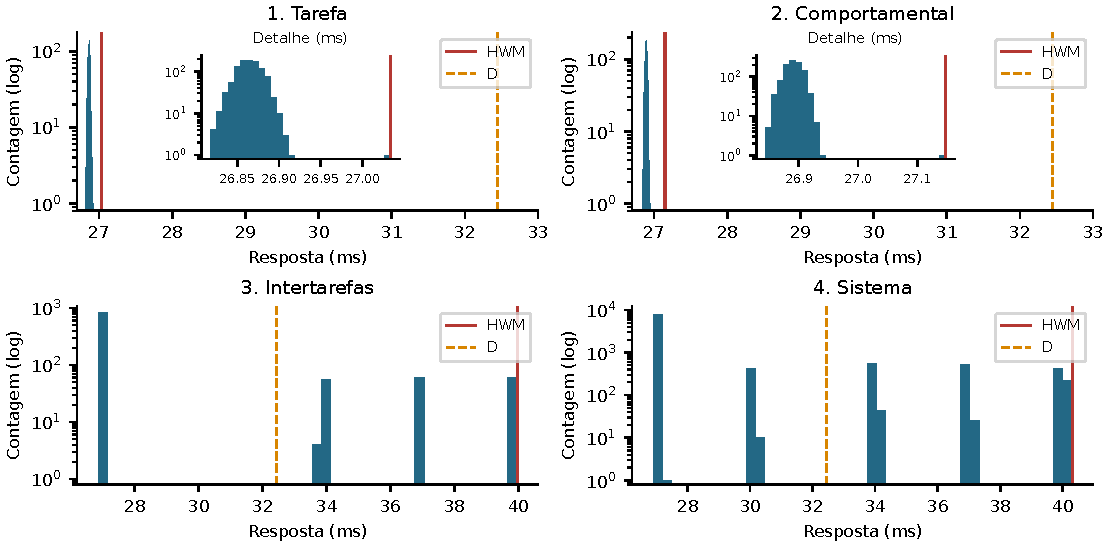
\includegraphics[width=\linewidth]{figuras/histogramas.pdf}
\par\vspace{3pt}
{\sffamily\fontsize{7.5}{10}\selectfont Figura 1 --- Histogramas das quatro coletas. HWM em vermelho; D em laranja. Nos dois primeiros painéis, o detalhe amplia a concentração abaixo de D. Eixo vertical logarítmico para mostrar também os valores raros.\par}
\vspace{7pt}

Nas etapas 1 e 2, as medianas são 26.865 e 26.891 \ensuremath{\mu}s, e os desvios padrão populacionais são 15,68 e 16,83 \ensuremath{\mu}s. A maioria dos valores fica muito próxima do centro; poucos tempos mais altos estendem a cauda à direita. O HWM supera o HWM99 em 136 e 224 \ensuremath{\mu}s, respectivamente, sem alcançar D.
\par

Nas etapas 3 e 4, as medianas permanecem próximas da referência (26.906 e 26.970 \ensuremath{\mu}s), mas os desvios padrão crescem para 3.977,56 e 3.997,67 \ensuremath{\mu}s. Surgem grupos próximos de 27, 30, 34, 37 e 40 ms. Não se trata apenas de uma cauda longa, fina e muito rara: diferentes condições de concorrência formam modos elevados. HWM\ensuremath{-}HWM99 vale 14 \ensuremath{\mu}s na etapa 3 e 210 \ensuremath{\mu}s na 4. A média, sozinha, oculta essa estrutura e as perdas.
\par

\clearpage

\section*{5. Evolução temporal, distâncias e rajadas}

\noindent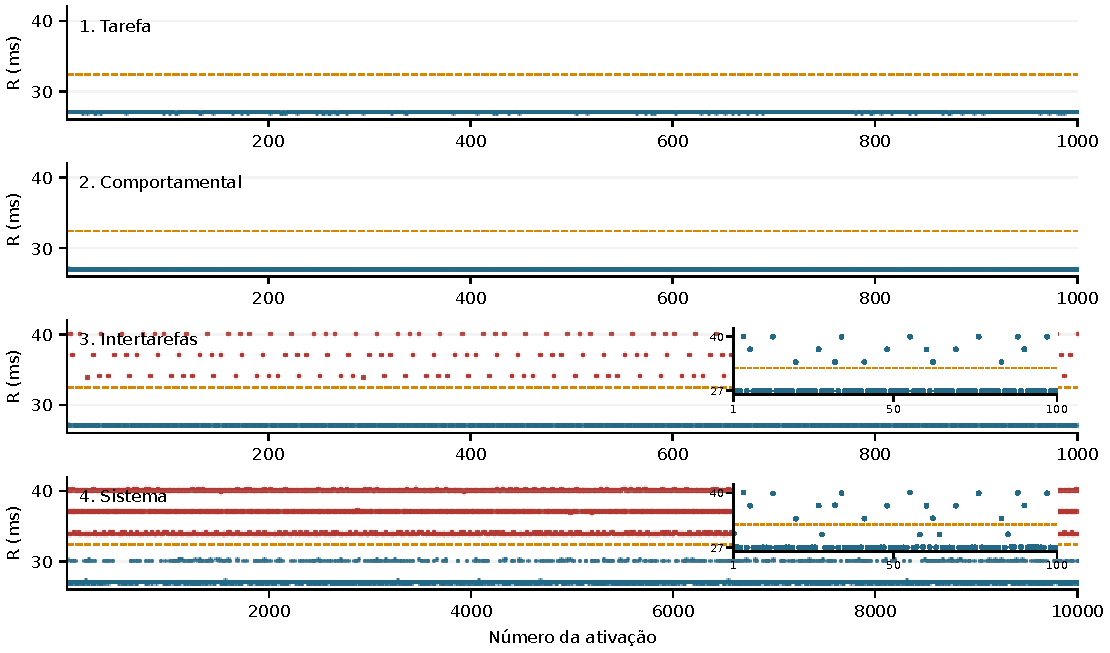
\includegraphics[width=\linewidth]{figuras/temporais.pdf}
\par\vspace{3pt}
{\sffamily\fontsize{7.5}{10}\selectfont Figura 2 --- Tempo de resposta por ativação. Vermelho marca R > D; a linha laranja indica D. Os quatro painéis usam a mesma escala vertical. Os detalhes das primeiras 100 ativações mostram a separação dos picos nas etapas 3 e 4.\par}
\vspace{7pt}

O atendimento de evento aumenta pouco o HWM da etapa 1 para a 2: de 27.034 para 27.148 \ensuremath{\mu}s. A inclusão de tarefas concorrentes eleva o máximo a 39.962 \ensuremath{\mu}s; com sistema e carga externa chega a 40.304 \ensuremath{\mu}s. Na escala completa, os pontos densos da etapa 4 parecem formar faixas. A análise pelos índices mostra, porém, que os picos acima do D fixo são isolados e recorrentes, sem perdas adjacentes. Nas etapas 1 e 2, o maior valor ocorreu na primeira ativação; possível efeito de primeira execução não foi instrumentado e não é tratado como causa comprovada.
\par

\begingroup
\fontsize{6.7}{8.8}\selectfont
\setlength{\tabcolsep}{3pt}
\renewcommand{\arraystretch}{1.25}
\noindent\begin{tabularx}{\linewidth}{@{}Y Y Y Y Y Y Y Y@{}}
\toprule
\rowcolor{cabecalho}
\textbf{Etapa} & \textbf{N} & \textbf{Perdas} & \textbf{Prazo (\%)} & \textbf{Isoladas} & \textbf{Rajadas} & \textbf{Maior seq.} & \textbf{S} \\
\midrule
1 & 1.000 & 0 & 100,00 & 0 & 0 & 0 & --- \\
2 & 1.000 & 0 & 100,00 & 0 & 0 & 0 & --- \\
3 & 1.000 & 179 & 82,10 & 179 & 0 & 1 & 2 \\
4 & 10.000 & 1.786 & 82,14 & 1.786 & 0 & 1 & 2 \\
\bottomrule
\end{tabularx}
\par\endgroup\vspace{5pt}

\textbf{Tabela 2 --- Perdas com D fixo.} Uma sequência máxima de tamanho 1 é isolada; uma rajada tem pelo menos duas perdas consecutivas. ``Maior seq.'' inclui as isoladas. S = mínimo(p[j+1] \ensuremath{-} p[j]), para índices de perda p em ordem de ocorrência.
\par

Nas duas últimas etapas, as primeiras perdas ocorrem nas ativações \textbf{4, 6, 13, 20, 27, 32, 34, 41, 48, 55, 60, 62, 69, \ldots{}}. As primeiras distâncias são \textbf{2, 7, 7, 7, 5, 2, 7, 7, 7, 5, 2, 7, \ldots{}}. Assim, S = 2: existe ao menos uma ativação cumprida entre quaisquer perdas consecutivas dessa amostra. S não é uma duração em milissegundos, e o período nominal não elimina o jitter.
\par

As listas integrais exigidas na seção 6.3 do enunciado acompanham o relatório: \path{analises/etapaN/perdas.csv} (índices, tempos e excesso), distancias.csv (cada par de perdas) e sequencias\_perdas.csv (início, fim, tamanho e classificação). Para as etapas 1--2, esses arquivos têm apenas cabeçalho, pois não há perdas. Esses anexos evitam substituir as 1.786 ocorrências da etapa 4 por uma seleção no texto.
\par

\clearpage

\section*{6. Análise específica de (m,k)-firme}

Uma exigência (m,k)-firme requer pelo menos m prazos cumpridos em \textbf{qualquer} janela de k ativações consecutivas. Para cada k \ensuremath{\in} \{10, 20, 50\}, percorremos todas as N\ensuremath{-}k+1 janelas completas, avançando uma ativação por vez. Se L(i,k) conta as perdas da janela iniciada em i, então m = k \ensuremath{-} máximo L(i,k). Não há janelas circulares nem preenchimento das bordas.
\par

\noindent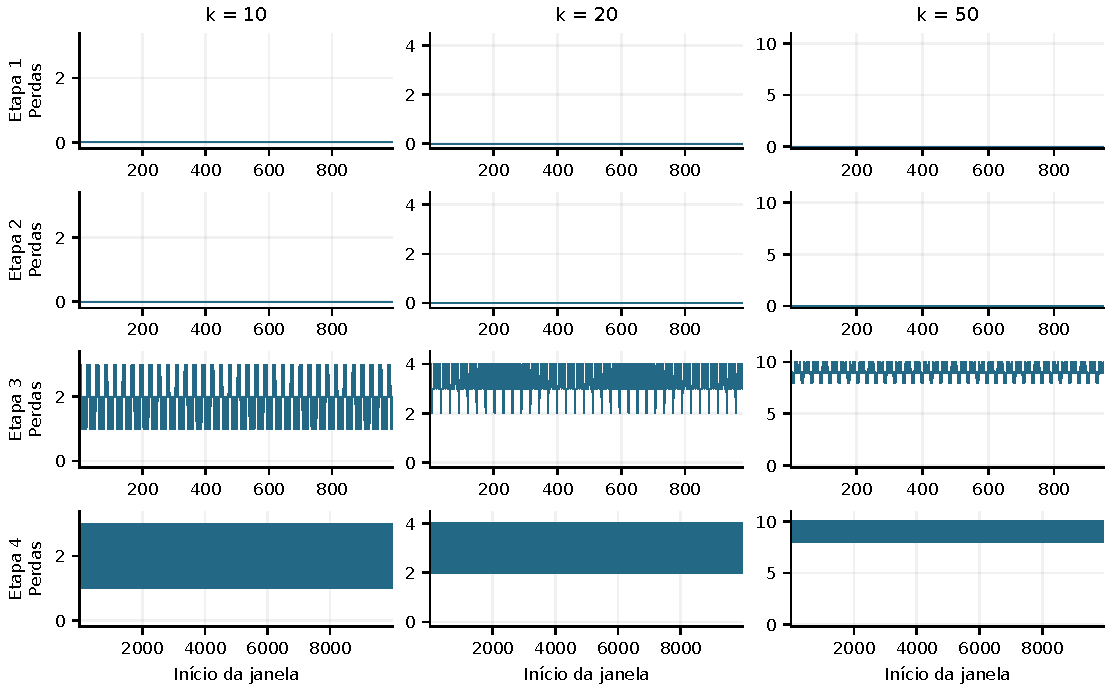
\includegraphics[width=\linewidth]{figuras/janelas.pdf}
\par\vspace{3pt}
{\sffamily\fontsize{7.5}{10}\selectfont Figura 3 --- Perdas por janela, com D fixo: linhas = etapas; colunas = k. Cada ponto usa todas as ativações da janela, sem subamostragem dos cálculos. A escala vertical é compartilhada em cada coluna.\par}
\vspace{7pt}

As etapas 1--2 exibem (10,10), (20,20) e (50,50): nenhuma janela contém perda. Nas etapas 3--4, os piores casos têm 3, 4 e 10 perdas, resultando em \textbf{(7,10), (16,20) e (40,50)}. Na janela [1,20] dessas duas etapas, as perdas 4, 6, 13 e 20 já testemunham o limite de quatro perdas. As tabelas completas janelas\_k10.csv, janelas\_k20.csv e janelas\_k50.csv acompanham cada etapa.
\par

Ter 82,14\% globalmente no prazo não garante 82,14\% em todo intervalo curto. A propriedade (16,20) fornece uma restrição local verificável sobre a sequência. Por outro lado, os três pares de uma etapa não são intercambiáveis: limitar perdas em 50 ativações não descreve sozinho a pior concentração em 10.
\par

\textbf{Limite da conclusão.} Os pares encontrados descrevem exclusivamente as janelas observadas. Não são prova de escalonabilidade nem garantia de cumprimento futuro. Sem conhecer todos os estados de execução e a relação com uma planta física, não se pode declarar a tolerância segura para um equipamento real.
\par

\clearpage

\section*{7. Experimentos A, B e C}

\subsection*{A --- Cobertura da lógica e máximo observado}

GCC/gcov 8.1.0 no Windows, com -O0 e --coverage, registrou \textbf{89/90 linhas (98,89\%) e 79/80 resultados de desvio (98,75\%)} de main/huffman.c. A suíte contém entradas vazias, símbolo único, todos os 256 símbolos, códigos longos, 1.000 entradas pseudoaleatórias, vetor conhecido e casos de erro. ``Branches executed = 100\%'' significa que as decisões foram alcançadas, não que todos os seus resultados foram exercitados.
\par

O resultado não alcançado é o erro de overflow na soma de bits. O limite de entrada UINT32\_MAX e códigos de até 255 bits não esgotam size\_t de 64 bits no teste; para os 4.096 bytes da campanha também não esgotam 32 bits. Mantivemos a proteção. Essa é a justificativa de impossibilidade permitida no enunciado. \textbf{Não houve marco de cobertura 100\% ao qual associar um HWM.} A cobertura foi medida separadamente dos tempos da placa; os fontes do módulo coincidem nas quatro etapas e no teste de cobertura.
\par

Ainda assim, o HWM passou por 27.034, 27.148, 39.962 e 40.304 \ensuremath{\mu}s sem mudar o algoritmo. Cobertura de linhas/desvios não é cobertura de todos os caminhos, nem enumera fases de interrupções, estados de cache ou bloqueios. Os dados mostram dependência do contexto temporal; não demonstram uma saturação experimental em 100\%.
\par

\subsection*{B --- Convergência do HWM}

\noindent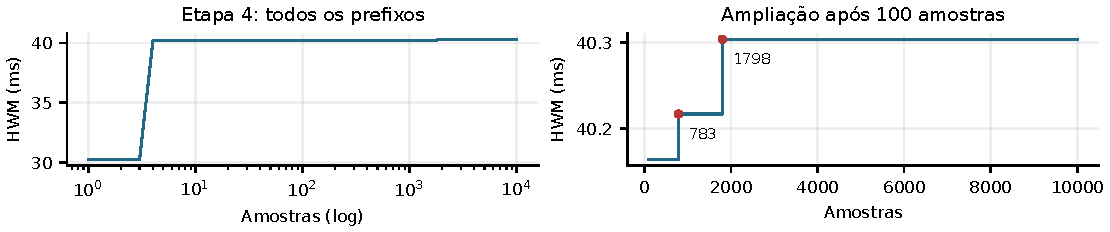
\includegraphics[width=\linewidth]{figuras/convergencia.pdf}
\par\vspace{3pt}
{\sffamily\fontsize{7.5}{10}\selectfont Figura 4 --- HWM acumulado da etapa 4: visão geral e ampliação a partir de 100 amostras. Os patamares são interrompidos por novos máximos.\par}
\vspace{7pt}

\begingroup
\fontsize{6.7}{8.8}\selectfont
\setlength{\tabcolsep}{3pt}
\renewcommand{\arraystretch}{1.25}
\noindent\begin{tabularx}{\linewidth}{@{}Y Y Y Y Y Y@{}}
\toprule
\rowcolor{cabecalho}
\textbf{N} & \textbf{10} & \textbf{20} & \textbf{100} & \textbf{1.000} & \textbf{10.000} \\
\midrule
HWM (\ensuremath{\mu}s) & 40.164 & 40.164 & 40.164 & 40.217 & 40.304 \\
\bottomrule
\end{tabularx}
\par\endgroup\vspace{5pt}

\textbf{Tabela 3 --- Máximos acumulados nos prefixos da etapa 4.}
\par

Com 10 ou 20 amostras, o HWM é 40.164 \ensuremath{\mu}s, apenas 0,347\% abaixo do máximo final: nesta coleta a subestimação inicial foi pequena. Esse patamar dura da ativação 4 até 782; na 783 sobe para 40.217 \ensuremath{\mu}s, valor ainda observado com 1.000 amostras. Na ativação 1.798 atinge 40.304 \ensuremath{\mu}s. A ausência de aumentos posteriores não prova convergência ao WCRT. Cada tamanho usa um prefixo da mesma coleta, não uma nova execução.
\par

\subsection*{C --- Margens sobre o HWM isolado}

\begingroup
\fontsize{6.7}{8.8}\selectfont
\setlength{\tabcolsep}{3pt}
\renewcommand{\arraystretch}{1.25}
\noindent\begin{tabularx}{\linewidth}{@{}Y Y Y Y@{}}
\toprule
\rowcolor{cabecalho}
\textbf{Margem} & \textbf{Limite (\ensuremath{\mu}s)} & \textbf{HWM4 \ensuremath{-} limite (\ensuremath{\mu}s)} & \textbf{Primeira etapa insuficiente} \\
\midrule
10\% & 29.737,4 & 10.566,6 & 3 \\
25\% & 33.792,5 & 6.511,5 & 3 \\
50\% & 40.551,0 & -247,0 & Nenhuma observada \\
\bottomrule
\end{tabularx}
\par\endgroup\vspace{5pt}

\textbf{Tabela 4 --- Margens e comparação com HWM4 = 40.304 \ensuremath{\mu}s.} As margens de 10\% e 25\% deixam de cobrir o máximo na etapa 3. A de 50\% cobre as quatro coletas, com apenas 247 \ensuremath{\mu}s de folga na última. A margem exata sobre o HWM1 para cobrir HWM4 seria 49,0863\%. Isso não a transforma em margem segura futura. Como no exemplo de 12--14 ms contra 10--16 ms discutido em aula [2], aumento da dispersão muda a incerteza, mesmo com centros semelhantes; aqui os desvios padrão e histogramas mostram essa mudança.
\par

\clearpage

\section*{8. Experimento D: deadlines alternativos}

Reprocessamos integralmente as etapas 3 e 4 com cinco deadlines: HWM1; D fixo; intermediário (27.034 + 40.094)/2 = 33.564 \ensuremath{\mu}s; HWM99 da etapa 4; e o mínimo da meta (18,20). Esta meta é \textbf{ilustrativa}, pois não foi fornecida uma tolerância física. As listas de perdas, distâncias, rajadas e janelas k = 10/20/50 de todos esses casos estão em \path{analises/experimento_d.} A tabela apresenta os três pares para permitir conferir também a repetição da análise 6.4.
\par

\begingroup
\fontsize{6.7}{8.8}\selectfont
\setlength{\tabcolsep}{3pt}
\renewcommand{\arraystretch}{1.25}
\noindent\begin{tabularx}{\linewidth}{@{}Y Y Y Y Y Y Y Y@{}}
\toprule
\rowcolor{cabecalho}
\textbf{Etapa} & \textbf{D (\ensuremath{\mu}s)} & \textbf{Prazo (\%)} & \textbf{S} & \textbf{k=10} & \textbf{k=20} & \textbf{k=50} & \textbf{I/R/M} \\
\midrule
3 & 27.034 & 82,00 & 2 & (7,10) & (15,20) & (40,50) & 180/0/0 \\
3 & 33.564 & 82,10 & 2 & (7,10) & (16,20) & (40,50) & 179/0/0 \\
3 & 40.094 & 100,00 & --- & (10,10) & (20,20) & (50,50) & 0/0/0 \\
3 & 32.440,8 & 82,10 & 2 & (7,10) & (16,20) & (40,50) & 179/0/0 \\
3 & 39.960 & 99,80 & 294 & (9,10) & (19,20) & (49,50) & 2/0/0 \\
4 & 27.034 & 66,87 & 1 & (0,10) & (7,20) & (25,50) & 1379/526/11 \\
4 & 33.564 & 82,14 & 2 & (7,10) & (16,20) & (40,50) & 1786/0/0 \\
4 & 40.094 & 99,00 & 2 & (8,10) & (18,20) & (47,50) & 100/0/0 \\
4 & 32.440,8 & 82,14 & 2 & (7,10) & (16,20) & (40,50) & 1786/0/0 \\
4 & 39.960 & 97,14 & 2 & (8,10) & (18,20) & (46,50) & 286/0/0 \\
\bottomrule
\end{tabularx}
\par\endgroup\vspace{5pt}

\textbf{Tabela 5 --- Variação de D (\ensuremath{\mu}s).} I/R/M = perdas isoladas / número de rajadas / tamanho da maior rajada (\ensuremath{\geq}2). S em ativações; ``---'' indica ausência de duas perdas. Para D = HWM99, 99,00\% cumprem o prazo na etapa 4: nesta amostra há exatamente 100 tempos estritamente acima do corte. A igualdade R = D é sempre considerada cumprimento.
\par

\noindent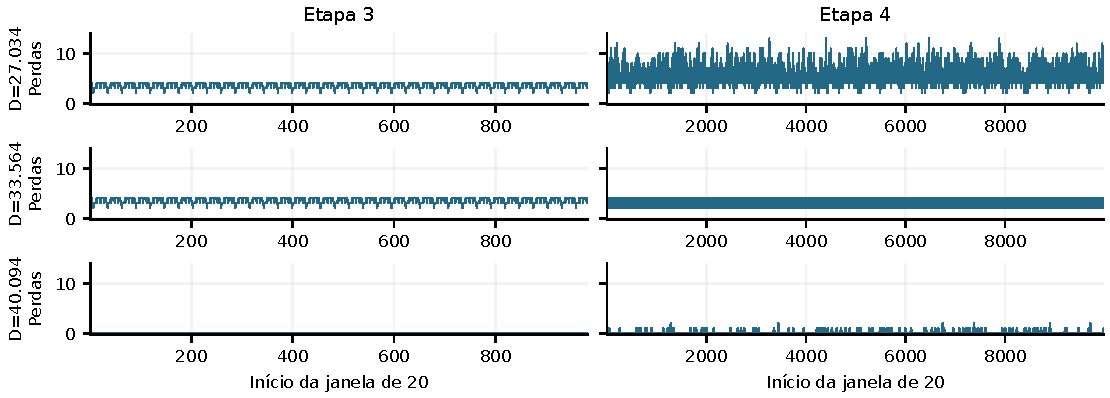
\includegraphics[width=\linewidth]{figuras/alternativos.pdf}
\par\vspace{3pt}
{\sffamily\fontsize{7.5}{10}\selectfont Figura 5 --- Janelas k = 20 para três deadlines alternativos nas etapas 3 e 4. As demais séries, incluindo k = 10 e 50, estão nos CSV e no caderno de gráficos.\par}
\vspace{7pt}

\textbf{Menor D para (18,20).} Em cada janela, tomamos o 18º menor dos 20 tempos; o máximo desses valores é o menor D que atende a todas as janelas. Na etapa 4, \textbf{D mínimo = 39.960 \ensuremath{\mu}s}. O tempo distinto imediatamente anterior, 39.957 \ensuremath{\mu}s, produz três perdas na janela [3431,3450], isto é, (17,20), e falha. O limiar encontrado resulta em 97,14\% no prazo e (18,20); comparado a D = HWM100 = 40.304 \ensuremath{\mu}s, reduz o prazo em 344 \ensuremath{\mu}s (0,854\%). Usar HWM100 elimina perdas apenas nesta amostra.
\par

\textbf{Perdas isoladas versus rajadas.} Com D = 27.034 \ensuremath{\mu}s, a etapa 4 apresenta 526 rajadas, a maior de 11 perdas, além de 1.379 isoladas; S cai para 1. Com o D fixo, as 1.786 perdas são isoladas. Em um sistema com inércia física, uma correção omitida pode ser tolerável, enquanto várias seguidas prolongam a ausência de atualização. Percentuais iguais podem esconder agrupamentos distintos; por isso, espaçamento, rajadas e janelas complementam a taxa global. A campanha não valida a estabilidade de uma planta física.
\par

\clearpage

\section*{9. Reprodutibilidade e evidências}

Os quatro CSV foram conferidos linha a linha contra os logs originais, com verificação dos hashes registrados. Há snapshots dos fontes e sdkconfig por etapa; o módulo Huffman e a configuração coincidem entre eles. As métricas usam nanossegundos inteiros nas comparações, evitando erro de igualdade com D. Os testes automatizados cobrem bordas das janelas, perdas isoladas/rajadas, descarte do HWM99 e o cálculo do deadline mínimo. Uma segunda implementação conferiu 14 cenários e 42 séries de janelas, incluindo a última janela de cada série.
\par

Na raiz do repositório, instalar requirements-relatorio.txt em ambiente Python e executar \path{scripts/analisar_coletas.py}, \path{scripts/verificar_analises.py} e \path{scripts/gerar_relatorio.py}, nessa ordem. Os testes usam python -m unittest discover -s tests -p test\_metricas.py -v. O README explica a reprodução; fontes por etapa estão em \path{dados/etapaN/fontes.} Reprocessar os CSV reproduz as tabelas; novas execuções podem produzir outros tempos.
\par

\textbf{Organização da entrega:} relatorio/ (PDF e texto editável); main/ (algoritmo e instrumentação); scripts/ e tests/; \path{dados/etapa1}--4/ (CSV, logs e snapshots); \path{dados/cobertura/} (gcov); analises/ (tabelas, séries de perdas/janelas e figuras). O código, os dados brutos e os resultados estão disponíveis no repositório indicado na primeira página.
\par

\section*{10. Ameaças à validade}

\textbf{Escopo e causalidade.} O intervalo da etapa 1 é de processamento; nas seguintes incorpora atendimento de evento e contenção. Essa ampliação é intencional, mas impede atribuir toda diferença a um único custo. O envio efetivo não captura o jitter anterior do gerador. Igualdade entre totais de contenções e perdas não é prova de correspondência individual. Retenção de mutex com espera representa a política de recurso simulada, não todo sistema embarcado.
\par

\textbf{Duração e entradas.} Existe uma campanha por cenário, com uma semente e um tamanho. A etapa 4 tem dez vezes mais amostras, o que também favorece encontrar máximos maiores. Limitando-a às primeiras 1.000, HWM = 40.217 \ensuremath{\mu}s e 82,10\% cumprem D, contra 39.962 \ensuremath{\mu}s e 82,10\% na etapa 3. A diferença persiste nessa comparação, mas não isola o efeito causal da UART nem substitui repetições independentes.
\par

\textbf{Plataforma e instrumentação.} Cache, interrupções e tarefas internas não foram rastreados por ativação. Frequência fixa e ausência de gerenciamento dinâmico não eliminam estados ocultos. Relógio e validação integram a medição; a saída serial foi adiada. Os tempos vêm de uma ESP32 com RTOS; o computador gerador da carga tem processos não controlados. Não foram avaliados outros sistemas operacionais ou arquiteturas. Os resultados se limitam à plataforma e às condições descritas.
\par

\textbf{Rastreabilidade e estresse.} O sufixo v6.1-dirty não identifica as alterações no SDK; sdkconfig igual não prova ambientes idênticos. Na etapa 2, houve 33.340 bytes ilegíveis/mensagens ROM antes do boot completo, sem marcadores da tarefa ou medições. O log bruto foi preservado; o sufixo válido contém uma execução completa e as 1.000 linhas, sem descarte de amostras, com SHA do ELF conferido. A causa do prefixo não foi determinada. Não há rastreamento de bytes UART perdidos por ativação. Rede, flash e outras cargas podem revelar tempos maiores. Cobertura não abrange o firmware inteiro; HWM e (m,k) não são garantias formais.
\par

\section*{11. Conclusão}

O teste isolado apresentou HWM de 27.034 \ensuremath{\mu}s e nenhuma perda no D fixo; o teste de sistema chegou a 40.304 \ensuremath{\mu}s, aumento de 49,09\%, com 17,86\% de perdas. A concorrência muda a distribuição mesmo sem alterar a lógica de Huffman. Cobertura elevada é evidência funcional, mas não esgota os estados temporais. Saltos tardios do máximo reforçam que um patamar observado não identifica o WCRT.
\par

O modelo (m,k) torna a tolerância verificável: com D fixo, as etapas 3 e 4 exibem (16,20), apesar de todas as perdas serem isoladas. A meta ilustrativa (18,20) exige D \ensuremath{\geq} 39.960 \ensuremath{\mu}s na sequência da etapa 4. Esse resultado, junto de S e das rajadas, descreve melhor a concentração das perdas que um percentual único, preservando a distinção entre evidência experimental e garantia futura.
\par

\subsection*{Referências}

[1] UNIVALI. Atividade Complementar --- Quanto o teste enxerga do pior caso. Sistemas em Tempo Real, M3. Enunciado fornecido, 6 p.
\par

[2] UNIVALI. Estimação do Tempo de Resposta usando Medições. Aula 10, material fornecido na disciplina, 39 p.
\par

\end{document}
